\documentclass{article}
\usepackage{PRIMEarxiv}
\usepackage[utf8]{inputenc}
\usepackage[T1]{fontenc}
\usepackage{amsmath,amssymb}
\usepackage{booktabs,array}
\usepackage[numbers,sort&compress]{natbib}
\usepackage{microtype}
\usepackage[hidelinks]{hyperref}
\usepackage{graphicx}
\pagestyle{fancy}
\fancyhead[L]{MARL under Limited Communication}
\fancyhead[R]{Final Report}
\title{Can Opponent Learning Compensate for Limited Communication?\\Multi-Agent Reinforcement Learning for Cooperative Pursuit}
\author{
  Piyush Choudhary \\ Roll No.: 23110247 \\ \texttt{piyush.choudhary@iitgn.ac.in}
  \And
  Shivansh Shukla \\ Roll No.: 23110303 \\ \texttt{shivansh.shukla@iitgn.ac.in}
}
\date{}
\begin{document}
\maketitle
\begin{abstract}
Four non-player characters (NPCs) pursue one player through a 20-by-20 corridor map using only local line-of-sight observations and a budgeted 16-byte broadcast channel. We build four pursuers: independent pursuit (IP), rule-based coordination (RC), communication-constrained recurrent MAPPO (MARL), and MAPPO with an explicit local opponent model (MARL-OM). We train 120 paired runs over three waypoint-player randomness levels, four communication budgets and five seeds, evaluate them against scripted and learning players, and report capture rate, capture time and actual communication with bootstrap uncertainty. Against the stationary and mildly random waypoint players every method captures almost every episode, so those conditions are ceiling results. Against the highly random player ($\xi=0.75$) MARL-OM captures 0.93 versus 0.82 for MARL at budget $1/8$ (gain $+0.11$, 95\% CI $-0.01$ to $0.22$), and on transfer to held-out Q-learning players the gain at $1/8$ is $+0.27$ (95\% CI $0.01$ to $0.58$); neither passes the pre-specified five-seed Holm test, so both are reported as estimates. Updating the predictor online shows no measurable difference from a frozen one.
\end{abstract}
\keywords{multi-agent reinforcement learning \and opponent modeling \and partial observability \and communication constraints \and pursuit--evasion}

\section{Introduction}
Imagine four NPCs pursuing a player through a corridor map. One sees the player turn left; the others see empty space. A message could tell them which route to cover, and when messages are scarce a pursuer that has learned the player's usual turns may still predict an interception point (Figure~\ref{fig:map}). We study when an explicit opponent model adds value on top of, or in place of, communication.

\begin{figure}[t]
\centering
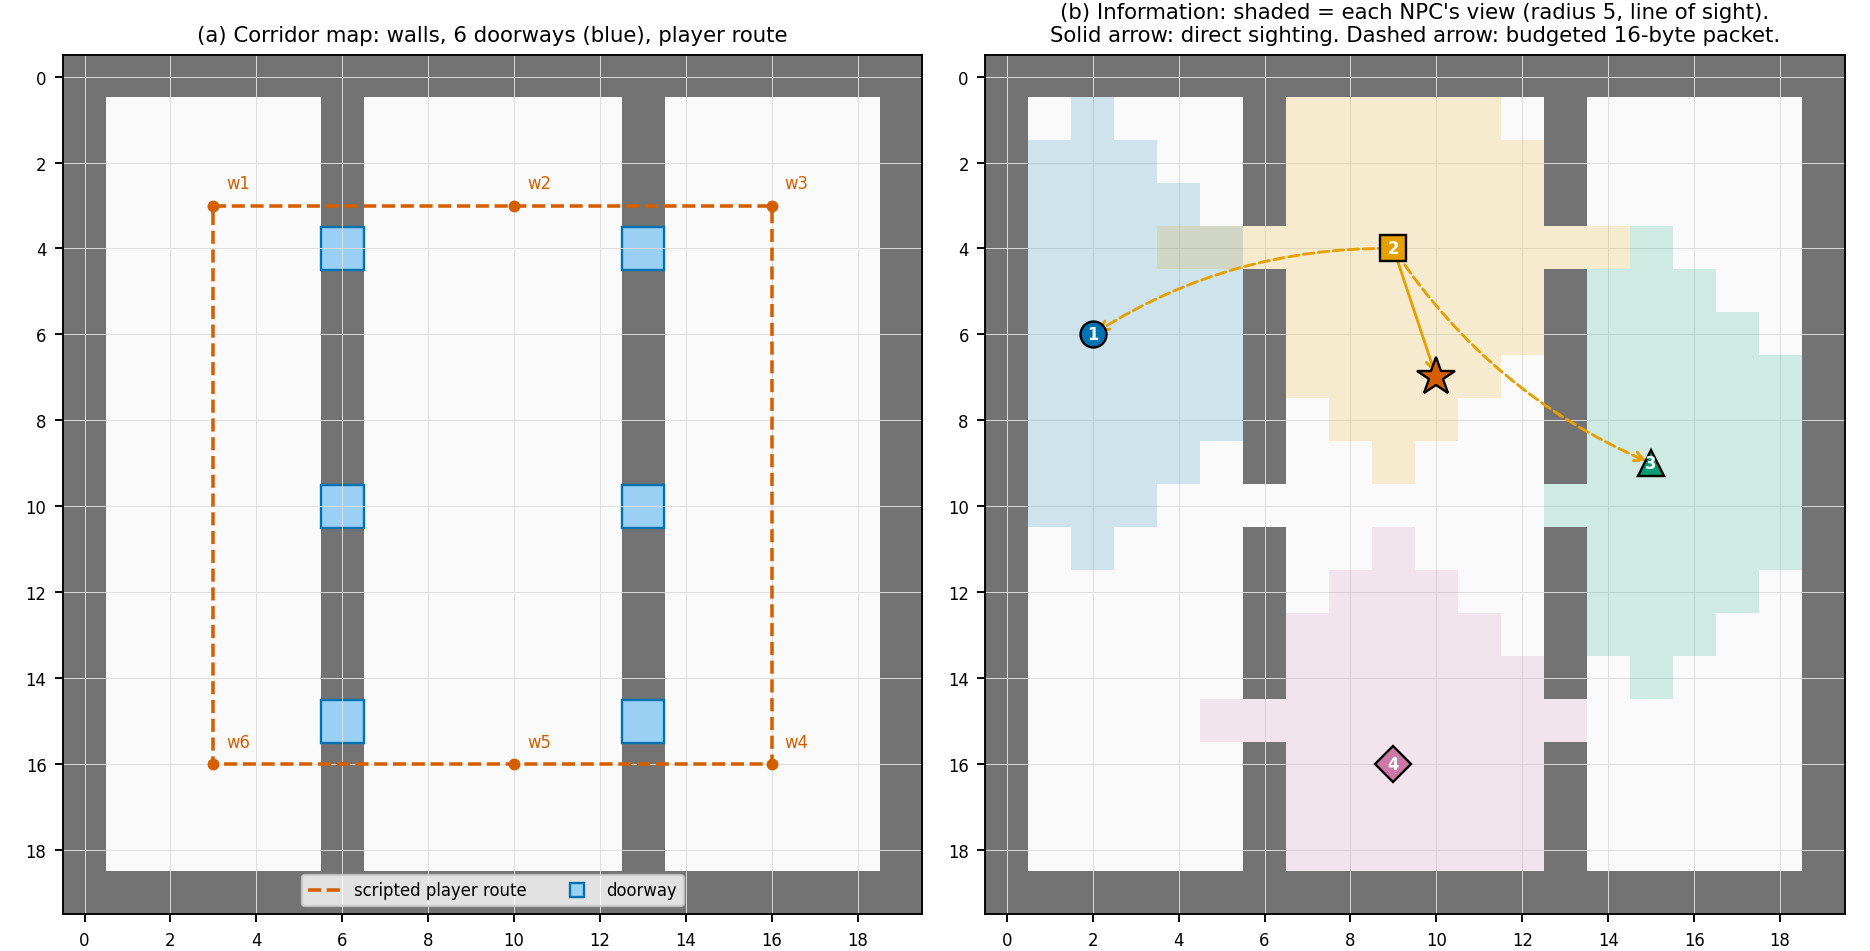
\includegraphics[width=\linewidth]{figures/map_information.png}
\caption{The corridor map and what each NPC can see: radius-5 line of sight, three rooms joined by doorways.}
\label{fig:map}
\end{figure}

We answer three questions: (1) how the communication budget affects capture; (2) at equal budget, whether explicit opponent modeling helps and how much communication it can replace; (3) whether the benefit holds when the player learns to evade, and whether updating the opponent model online helps track that change.

\section{Background and preliminaries}
Distributed constraint optimization (DCOP) supports role and task allocation \citep{fioretto2018}; our rule-based coordinator uses a local utility-with-overlap score in that spirit. Multi-agent reinforcement learning (MARL) provides the sequential decision framework; we use recurrent MAPPO with a centralized critic \citep{yu2022}. Opponent modeling predicts the player's next move \citep{albrecht2018}. The player has its own learning algorithm. These components are kept separate throughout. Notation: $N=4$ NPCs, horizon $H=200$, budget $B\in\{0,\tfrac18,\tfrac12,1\}$ packets per NPC per step, waypoint randomness $\xi$, $P_{\text{MARL}}(B)$ and $P_{\text{OM}}(B)$ capture rates, and $G(B)=P_{\text{OM}}(B)-P_{\text{MARL}}(B)$.

\section{Problem formulation}
\textbf{Environment.} A 20$\times$20 grid with walls at the boundary and at columns 6 and 13 (doorways at rows 4, 10 and 15). Four NPCs and one player move one cardinal cell per step; all moves resolve simultaneously. Capture is co-location after movement or an opposite-direction swap. An episode lasts at most $H=200$ steps and ends on capture.

\textbf{Information.} Each NPC sees cells within Manhattan distance 5 that have a clear line of sight (supercover traversal; a wall touched at a corner blocks sight). NPCs know the map, their ID, time, budget and radius, but not the player's position unless it is visible or reported.

\textbf{Channel.} A budget $B\in\{0,1/8,1/2,1\}$ allows NPC $i$ to send at decision $t$ only if $\mathrm{sent}_i<\lfloor B(t+1)\rfloor$. A packet is a fixed 16-byte broadcast delivered at the next decision and charged even if capture occurs on that transition.

\textbf{Reward.} $r=\mathbf 1[\text{capture}]-0.10/H-0.01\,b_t/(NH)-0.02\,m_t/(NH)$ with $\gamma=1$, where $b_t$ is the number of broadcasts and $m_t$ the number of NPC moves at step $t$.

\section{Methodology}
We compare four pursuers that differ in how they combine local sight, messages and a model of the player. All four act decentrally: an NPC's decision uses only its own observation, its memory and the packets delivered to it.

\subsection{Rule-based pursuers}
\textbf{Independent pursuit (IP).} Each NPC walks a shortest path to the latest cell where it directly saw the player; when it has none it searches its own quadrant of the map. IP never sends.

\textbf{Rule-based coordination (RC).} Each NPC keeps a memory of the newest sighting (its own or received) and shares a role hint: chase, intercept, block or search. The role and its destination come from a local utility score with an overlap penalty, in the spirit of DCOP task allocation \citep{fioretto2018}, so that teammates do not all pick the same destination. An NPC sends when it makes a new sighting, when its role or destination changes, or every ten steps, always subject to the budget rule of Section~3. A packet carries sender, flags, sender cell, target cell, target step, displacement, role, destination and send step in 16 bytes.

\subsection{MARL: communication-constrained recurrent MAPPO}
The learned pursuers share one actor network across the four NPCs and are trained with multi-agent PPO using a centralized critic \citep{yu2022}. The actor reads a five-channel $20\times20$ local map (walls, cells currently visible, own position, visible teammates and the cell where the player is directly seen) through two $3\times3$ convolutions (16 and 32 channels) and a linear layer to 64 units. It concatenates this with a vector of scalar features (NPC identity, remaining time, budget, available send credit, previous move and send, the newest sighting held in memory with its age and displacement, the current role and destination, and the latest packet from each teammate) and passes the result through a 64-unit GRU cell. The head outputs ten logits, one for each of five moves crossed with send or stay silent. Budget-illegal sends are masked, so an NPC cannot exceed its allowance. At execution the actor takes the greedy action.

The centralized critic is a 128--128 MLP on the full state (all positions, the map, channel credit and usage, time and the training opponent's controller state). It is used only for training and never at execution. Training uses the reward of Section~3 with $\gamma=1$, GAE $\lambda=0.95$, clip 0.2, value coefficient 0.5, entropy coefficient 0.01, learning rate $3\times10^{-4}$, gradient-norm clip 0.5, 8 parallel environments, 128-step rollouts, 4 epochs over 16-step sequences in 4 minibatches. A short curriculum draws closer player starts (distance 1--3, then 4--8) during the first 90k transitions. Every run trains for exactly 1.2M environment transitions and the final checkpoint is evaluated; no best-checkpoint selection is used.

\subsection{MARL-OM: adding a local opponent model}
MARL-OM adds, for each NPC, a small predictor and a belief that never see the player's hidden state. The predictor is a 42--32--32--5 MLP that outputs a distribution over the player's next displacement (four moves or stay). Its input holds the previous displacement, the region of the target cell, the NPC's position relative to the target and the visible teammates. It is trained with cross-entropy (Adam, learning rate $10^{-3}$, FIFO buffer of 512, five updates per rollout, batches of 64) only on labels that the NPC is permitted to observe: consecutive direct sightings.

Each NPC keeps a belief over (free cell, previous displacement). At each step the belief is propagated through the predictor, cells the NPC can see to be empty are removed, and a direct sighting or a received report collapses it. Seven summary features go to the actor: the mean and variance of the position in each axis, their covariance, the normalized entropy and the maximum probability. All other inputs, the architecture, the seeds and the training schedule are identical to MARL, so the comparison isolates the opponent model.

\subsection{Players and evaluation protocol}
\textbf{Waypoint player.} Cycles through a fixed list of waypoint cells along shortest paths; with probability $\xi\in\{0,0.25,0.75\}$ it takes a random legal move. \textbf{Q-learning player.} A tabular learner on a coarse local state ($\alpha=0.10$, $\gamma=0.95$, $\epsilon=0.10$); eight banks were trained (seeds 7000--7002 for validation, 7100--7104 held out).

\textbf{Experiment design.} Pursuers are trained against the waypoint player at the three $\xi$ levels, for four budgets and five seeds each (1000--1004), giving 120 runs; every run is evaluated on 100 held-out scenarios (scenario seeds from 100000). Pursuers trained at $\xi=0.75$ are then evaluated without retraining against the held-out Q-learning banks, in 20-episode blocks in which the player is frozen or keeps learning, and with the predictor frozen or updated online. The Q-learning player is used only for evaluation: during the pilot, training against it did not reach the adequacy criterion (capture of at least 0.20) in any variant.

\textbf{Statistics.} Capture rates are averaged over scenarios and then seeds. Intervals are 95\% percentile bootstrap intervals (5,000 resamples, seed 40000) that resample training seeds and then scenarios, paired across the two methods. The confirmatory test is a sign-flip test of $G(1/8)$ across seeds with Holm adjustment over conditions. Gap fractions whose denominator is zero are reported as undefined, and ceiling conditions are labelled uninformative rather than summarized.

\begin{figure}[t]
\centering
\fbox{\begin{minipage}{0.94\linewidth}\small
\textbf{Procedure (per run).}\
1. Fix $(\xi, B, \text{method}, \text{seed})$; initialize actor, critic and, for MARL-OM, the predictors.\
2. Repeat until 1.2M transitions: collect 8 environments $\times$ 128 steps with the masked actor; (MARL-OM) update beliefs from received packets and permitted sightings.\
3. Compute GAE from the centralized critic; run 4 PPO epochs on 16-step sequences; (MARL-OM) run 5 predictor updates per NPC.\
4. Evaluate the final checkpoint on 100 held-out scenarios (frozen waypoint), and for $\xi=0.75$ against held-out Q banks.
\end{minipage}}
\caption{Training and evaluation procedure for one learned run.}
\label{fig:proc}
\end{figure}

\section{Experimental setup and pilot}
All learned runs use 1.2M environment transitions. The pilot examined 300k, 600k and 1.2M steps. A revised adequacy check requires finite losses, at least 100 training captures, final validation capture of at least 0.20, and an improvement of at least 0.10 over the untrained policy. All six required waypoint conditions satisfy it (Table~\ref{tab:adequacy}).

\begin{table}[t]
\centering
\caption{Pilot adequacy at 1.2M transitions (median of two seeds, 100 validation episodes).}
\label{tab:adequacy}
\begin{tabular}{llrrr}
\toprule
Condition & Method & Capture & Gain vs.\ untrained & Change 800k$\to$1.2M \\
\midrule
$\xi=0$, $B=1$ & MARL & 1.00 & 0.48 & 0.00 \\
$\xi=0$, $B=1$ & MARL-OM & 1.00 & 0.48 & 0.00 \\
$\xi=0.75$, $B=1/8$ & MARL & 0.76 & 0.27 & $-0.01$ \\
$\xi=0.75$, $B=1/8$ & MARL-OM & 0.88 & 0.41 & $+0.06$ \\
$\xi=0.25$, $B=0$ & MARL & 1.00 & 0.55 & 0.00 \\
$\xi=0.25$, $B=0$ & MARL-OM & 1.00 & 0.57 & 0.00 \\
\bottomrule
\end{tabular}
\end{table}

\textbf{Task calibration.} Before fixing the task we audited message use (no packets at $B=0$; delivered packets update the receiver's memory and role hint) and compared four predeclared task variants on validation seeds. RC captured 97--100\% of episodes at $B=0$ in all four, so the original task (radius 5, $H=200$) is retained as the main task. The study therefore measures when communication and opponent prediction add value when strong baselines already capture nearly every episode.

\textbf{Baselines.} Against the waypoint players, IP and RC both capture every evaluation episode at every budget; IP, which sends nothing, finishes in fewer steps (17.0 versus 22--24 at $\xi=0$).

\section{Controlled results}
All 120 runs (3 waypoint levels $\times$ 4 budgets $\times$ 2 learners $\times$ 5 seeds) finished at 1.2M transitions. Each cell below is the mean over five training seeds, each evaluated on 100 held-out scenarios; intervals are 95\% paired bootstrap intervals (5,000 resamples). $G(B)=P_{\text{OM}}(B)-P_{\text{MARL}}(B)$ is the capture gain from the opponent model.

\textbf{Deterministic and mildly random players.} At $\xi=0$ and $\xi=0.25$ both learners capture essentially every episode at every budget (capture 0.996--1.000; Table~\ref{tab:ceiling}). Because capture is at ceiling, these two conditions do not separate the methods and are reported as uninformative for the gain and communication-saved measures; their gap fractions are left undefined rather than imputed.

\begin{table}[t]
\centering
\caption{Capture rate at $\xi\in\{0,0.25\}$ (mean over 5 seeds). IP and RC capture every episode at every budget.}
\label{tab:ceiling}
\begin{tabular}{llcccc}
\toprule
$\xi$ & Method & $B=0$ & $B=1/8$ & $B=1/2$ & $B=1$ \\
\midrule
0 & MARL & 1.000 & 1.000 & 1.000 & 1.000 \\
0 & MARL-OM & 1.000 & 0.998 & 1.000 & 1.000 \\
0.25 & MARL & 1.000 & 0.996 & 1.000 & 1.000 \\
0.25 & MARL-OM & 1.000 & 1.000 & 1.000 & 1.000 \\
\bottomrule
\end{tabular}
\end{table}

\textbf{Highly random player ($\xi=0.75$).} This is the only waypoint condition with headroom. MARL-OM captures more than MARL at $B=0$ (0.922 versus 0.860) and $B=1/8$ (0.932 versus 0.820), with $G(1/8)=+0.112$ (95\% CI $-0.006$ to $0.218$). At $B=1/2$ the order reverses ($G=-0.100$, CI $-0.280$ to $0.064$) and at $B=1$ the two are close ($G=+0.014$). The pre-specified test on $G(1/8)$ across five seeds gives a Holm-adjusted $p=0.56$ (the smallest attainable with five seeds is $0.0625$); the seed-level differences are $+0.18,+0.21,+0.23,-0.08,+0.02$. The point estimate favours MARL-OM at low budget, and the data do not establish it at the five-seed level.

\begin{table}[t]
\centering
\caption{Capture rate at $\xi=0.75$ (mean over 5 seeds; 95\% bootstrap interval).}
\label{tab:wp}
\begin{tabular}{lcccc}
\toprule
$B$ & MARL & MARL-OM & $G$ & 95\% CI for $G$ \\
\midrule
0 & 0.860 & 0.922 & $+0.062$ & $[-0.054,\,0.174]$ \\
1/8 & 0.820 & 0.932 & $+0.112$ & $[-0.006,\,0.218]$ \\
1/2 & 0.842 & 0.742 & $-0.100$ & $[-0.280,\,0.064]$ \\
1 & 0.820 & 0.834 & $+0.014$ & $[-0.068,\,0.090]$ \\
\bottomrule
\end{tabular}
\end{table}

\begin{figure}[t]
\centering
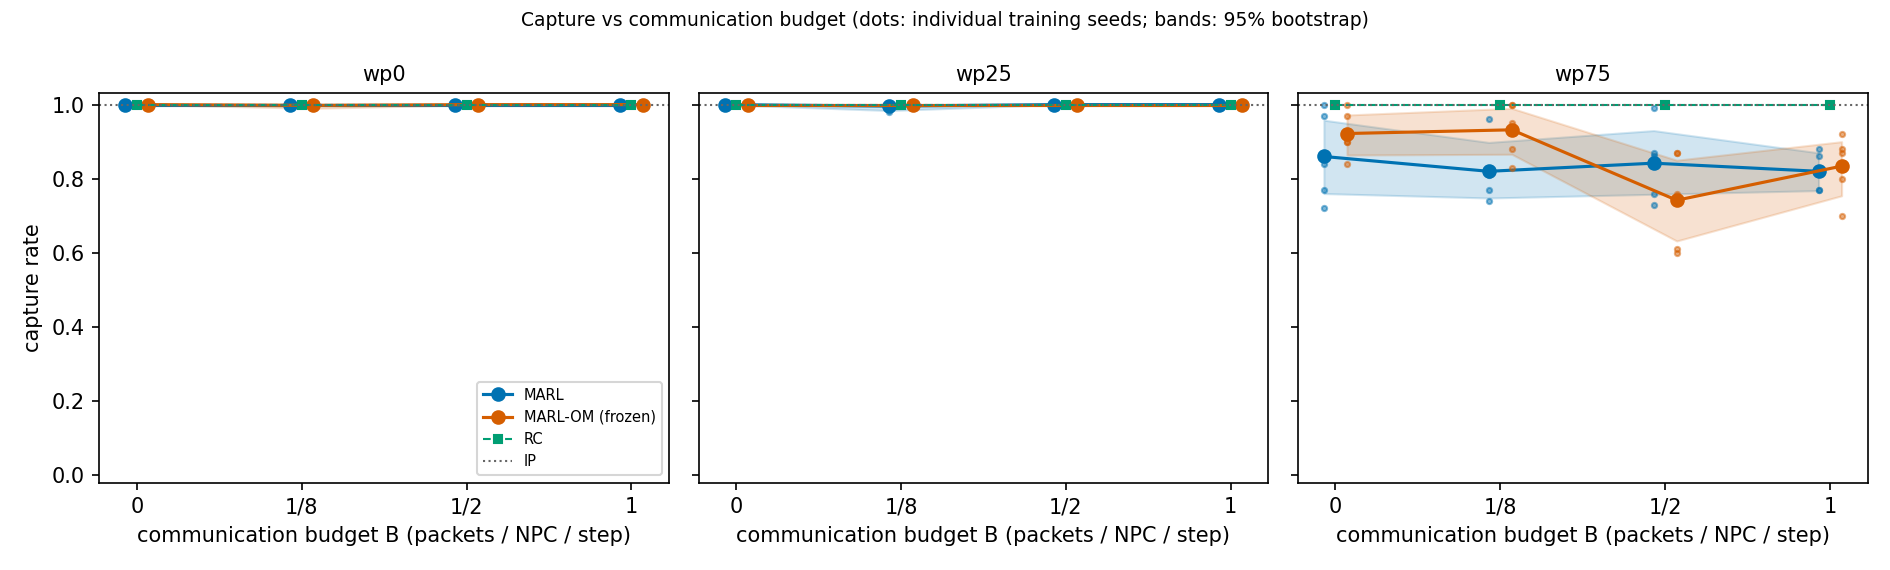
\includegraphics[width=\linewidth]{figures/capture_vs_budget_waypoint.png}
\caption{Capture rate versus communication budget against the waypoint player. Small dots are training seeds; bands are 95\% bootstrap intervals. IP and RC capture every episode.}
\label{fig:budget}
\end{figure}

\begin{figure}[t]
\centering
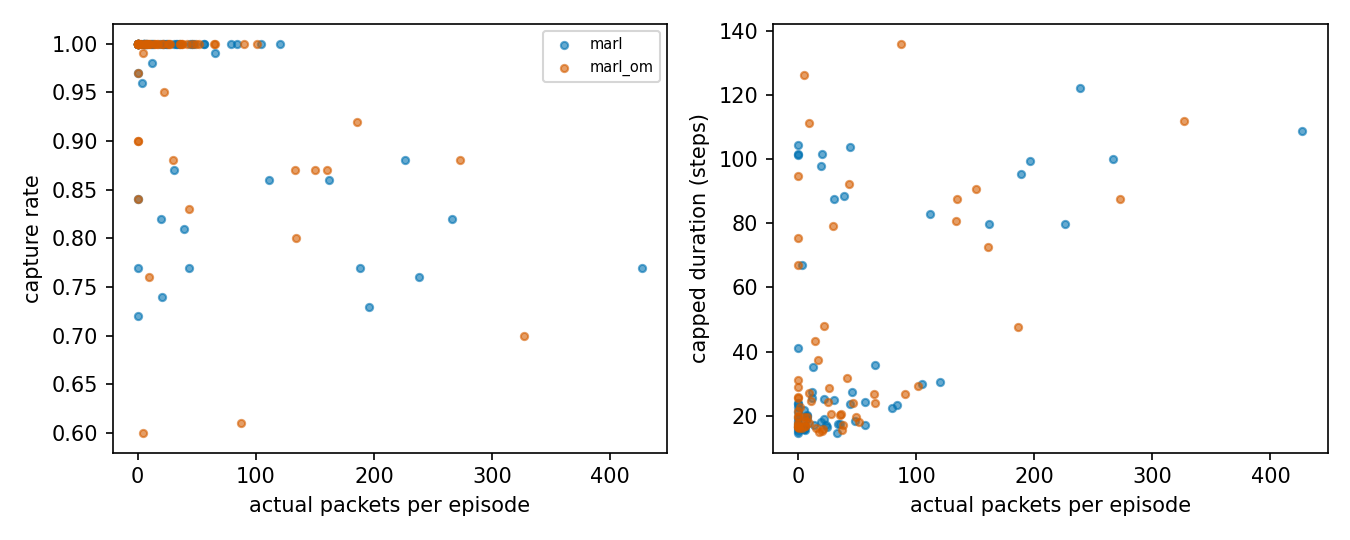
\includegraphics[width=\linewidth]{figures/packets_vs_capture.png}
\caption{Actual packets sent per episode against capture rate (left) and capped episode duration (right), one point per run and condition.}
\label{fig:packets}
\end{figure}

\textbf{Shuffled-feature control.} To check whether the predictor's content matters, we trained the MARL-OM architecture with its predictor features shuffled (10 extra runs, $B=1/8$, five seeds each at $\xi=0$ and $\xi=0.75$). At $\xi=0$ both capture every episode (1.000 versus 0.998). At $\xi=0.75$ the intact MARL-OM captures 0.932 and the shuffled variant 0.832, a difference of $+0.100$ with seed-level differences of $+0.29,-0.01,+0.11,+0.18,-0.07$; this control was not part of the confirmatory tests and is descriptive.

\textbf{Reliance on received messages.} To test whether trained pursuers use what they receive, we replayed the $B=1$, $\xi=0.75$ checkpoints on the same 100 scenarios with and without delivered packets reaching the receivers' memory. Capture is essentially unchanged: MARL 0.820 with packets and 0.828 without; MARL-OM 0.834 with and 0.828 without (per-seed differences between $-0.03$ and $+0.04$). The trained pursuers at this budget do not measurably depend on received messages in this task.

\textbf{Role of communication.} In this task the scripted baselines and the learners capture nearly every episode with no communication at $\xi\le0.25$, so extra messages have no capture headroom to add there. At $\xi=0.75$ capture does not increase monotonically with the budget for either learner (MARL: 0.860, 0.820, 0.842, 0.820), so the study does not show a budget-driven improvement in this setting.

\section{Adaptive-player results}
Pursuers trained against the $\xi=0.75$ waypoint player were evaluated, without retraining, against the held-out Q-learning player banks (an out-of-distribution transfer test, five held-out banks). Capture is low in absolute terms for both learners (Table~\ref{tab:q}), well below the 0.82--0.93 reached against the waypoint player the pursuers were trained on.

\begin{table}[t]
\centering
\caption{Transfer to the held-out Q-learning player (mean over 5 seeds; 95\% bootstrap interval).}
\label{tab:q}
\begin{tabular}{lcccc}
\toprule
$B$ & MARL & MARL-OM & $G$ & 95\% CI for $G$ \\
\midrule
0 & 0.240 & 0.372 & $+0.132$ & $[-0.280,\,0.548]$ \\
1/8 & 0.094 & 0.362 & $+0.268$ & $[0.010,\,0.584]$ \\
1/2 & 0.132 & 0.042 & $-0.090$ & $[-0.260,\,0.014]$ \\
1 & 0.064 & 0.162 & $+0.098$ & $[0.008,\,0.210]$ \\
\bottomrule
\end{tabular}
\end{table}

\begin{figure}[t]
\centering
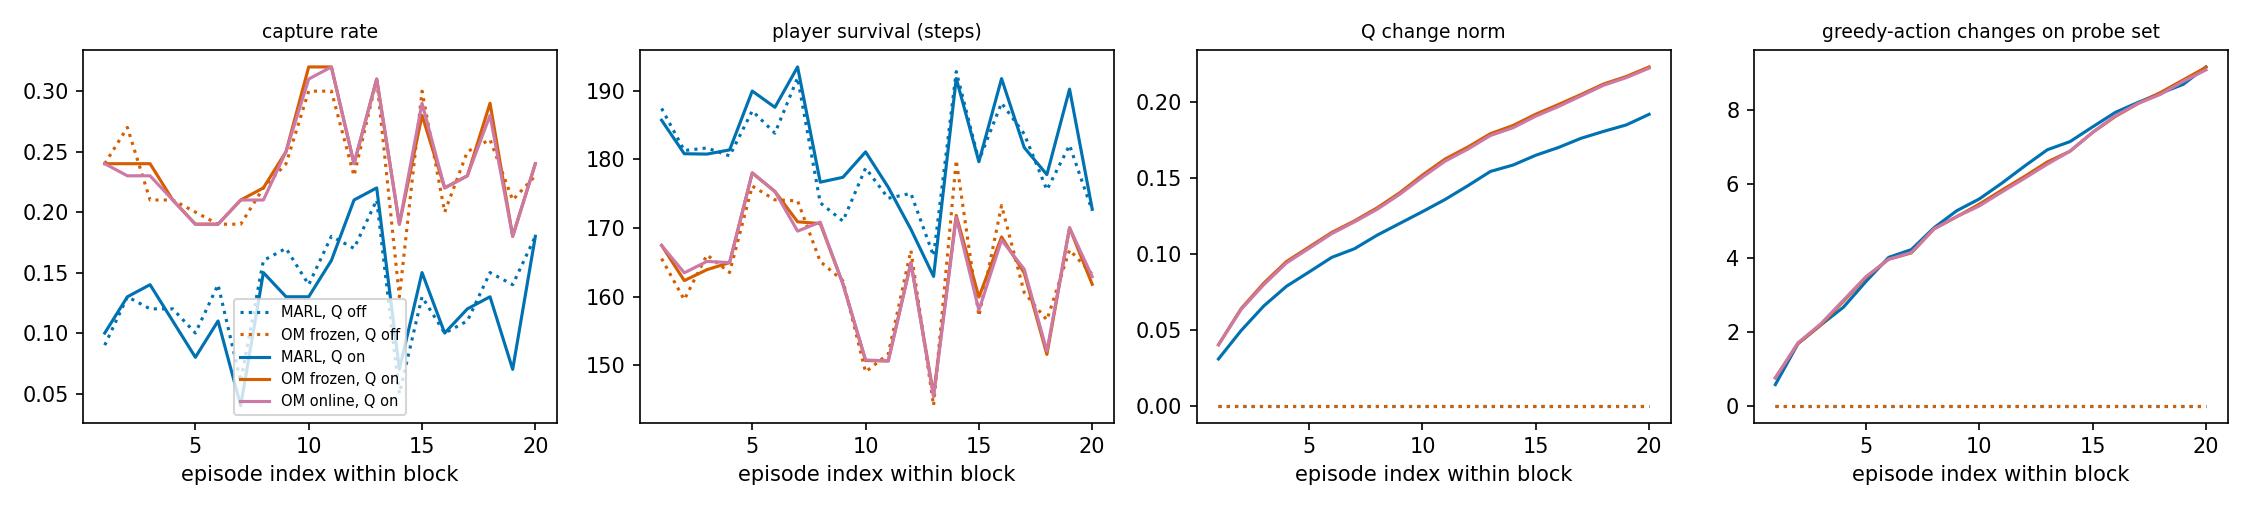
\includegraphics[width=0.9\linewidth]{figures/adaptive_curves.png}
\caption{Episode-index capture curves for the Q-learning player (exploratory): frozen versus online predictor.}
\label{fig:adaptive}
\end{figure}

At $B=1/8$ MARL-OM captures 0.362 versus 0.094 for MARL, and the interval for $G(1/8)$ excludes zero ($+0.268$, 95\% CI $0.010$ to $0.584$). The pre-specified five-seed sign-flip test gives a Holm-adjusted $p=0.19$, so the effect is a suggestive estimate rather than a confirmed one; per-seed differences are $+0.31,+0.25,+0.86,-0.10,+0.02$. As in the waypoint results, the sign flips at $B=1/2$ ($G=-0.090$).

\textbf{Tracking within a block.} Within the 20-episode adaptation blocks, capture in the first five and last five episodes is nearly unchanged for both methods: MARL 0.112$\to$0.136 (player frozen) and 0.112$\to$0.120 (player learning); MARL-OM 0.226$\to$0.230 (frozen) and 0.224$\to$0.232 (learning). Updating the predictor online gives 0.220$\to$0.230 against 0.224$\to$0.232 for the frozen predictor on the same blocks, so the two predictors differ by 0.002 or less in either window. These blocks show no measurable adaptation or tracking effect in either direction, and this analysis is exploratory.

\section{Discussion and limitations}
\textbf{What the measurements support.} (i) Strong scripted pursuers (IP, RC) and both learners capture nearly every episode against the stationary and mildly random players with no communication, so those conditions are ceiling results. (ii) Where headroom exists ($\xi=0.75$ and the Q-learning player), MARL-OM has the higher point estimate at $B=0$ and $B=1/8$; at $B=1/8$ against the Q-learning player the bootstrap interval for the gain excludes zero ($+0.268$). (iii) Neither gain survives the pre-specified five-seed Holm test (adjusted $p=0.56$ and $0.19$), so we report them as estimates with uncertainty. (iv) Online updating of the predictor shows no measurable difference from the frozen predictor within 20-episode blocks.

\textbf{Limits.} The main task was kept at radius 5 and $H=200$ after calibration showed RC at 97--100\% capture without messages in all four predeclared variants; the study therefore addresses communication in a task where it adds little to the strongest baselines, and a harder communication bottleneck is future work. The learned pursuers capture 0.82--0.93 against the $\xi=0.75$ player, below IP and RC, which capture every episode there. The Q-learning player is used only for evaluation, so its results measure transfer, not training against a learning opponent. Five seeds limit the attainable significance (smallest sign-flip $p=0.0625$).

\section{Contributions and reproducibility}
\begin{table}[h]
\centering
\caption{Task assignment and outcome.}
\label{tab:contrib}
\small
\begin{tabular}{p{2.3cm}p{8.2cm}p{2.6cm}}
\toprule
Member & Assigned tasks & Outcome \\
\midrule
Piyush Choudhary & Simulator, maps, capture, visibility and channel; waypoint and Q-learning players; IP and RC pursuers; environment tests; rendering and replay viewer & Fulfilled \\
Shivansh Shukla & Recurrent MAPPO; local predictors and beliefs; frozen, adaptive and online protocols; pilot and manifests; statistics and plots & Fulfilled; Q-player training scoped to evaluation-only transfer after the pilot \\
Both & Interfaces, protocol freeze, 120-run experiment, analysis, report, demo & Fulfilled \\
\bottomrule
\end{tabular}
\end{table}

\textbf{Reproducibility.} The code, configurations, run manifest, per-run evaluation outputs, analysis tables and figures are in the repository (\texttt{README.md} maps each table and figure of this report to the command and file that produces it). Every number in Tables~\ref{tab:ceiling}--\ref{tab:q} and Figures~\ref{fig:budget}--\ref{fig:adaptive} is computed by \texttt{python -m pursuit.cli analyze} from the saved per-run CSV files.

\bibliographystyle{plainnat}
\bibliography{references}
\end{document}
